
\subsection{View}

The engine is designed to assist the user in all parts of the process
when making an environment, this also extends to the visualization
of said environment. However, since our goal is to have as few restrictions
on the model as possible, our knowledge of that view\textquoteright{}s
representation is very limited.


\subsubsection{Concept}

The view API which the engine provides consists of four abstract classes
that are meant to be implemented by the user. The four classes can
be seen in fig. \ref{fig:ViewUMLView}. We will go through each class
and explain how they are meant to be implemented.

\begin{figure}
\begin{centering}
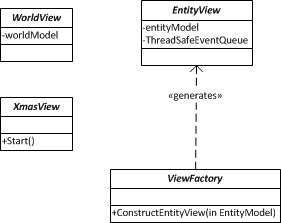
\includegraphics[width=0.7\textwidth]{ViewUmlDomainDiagram}
\par\end{centering}

\caption{UML diagram of the view\label{fig:ViewUMLView}}
\end{figure}



\paragraph*{\texttt{XmasView}}

The \texttt{XmasView} class is very simple; it only provides a single
method that is required to be implemented. When the engine starts
the view up it generates a thread for the view and the \texttt{Start}
method is the first method to be executed inside that thread. The
start method should contain an endless loop that on a time interval
updates the view. Another task of the implemented view is also to
update its \texttt{ThreadSafeEventManager.} The \texttt{ThreadSafeEventManager}
ensures that events sent from the model thread of the engine is not
immediately executed, but instead lie dormant in the \texttt{ThreadSafeEventManager}
until the view thread is ready to execute them. How many events that
one wishes to trigger is up to the user. We also provide the appropriate
methods for the user to specify exactly how long he wishes to wait
for the next event, or if it should timeout. The \texttt{ThreadSafeEventManager}
is very important to the view as without it, designing view code becomes
complicated as one need to constantly ensure that no concurrency bugs
has been applied to the system.


\paragraph*{\texttt{WorldView}}

The \texttt{WorldView} class is added because of the long term benefits,
as of now it provides nothing for the designer. However if we found
benefits to add to the class, making it ahead of time, even if it
is initially empty, can have many benefits as the project expands.


\paragraph*{\texttt{EntityView}}

Much like the \texttt{WorldView} class, the \texttt{EntityView} is
also very minimal. However, it enforces certain things that the user
of the engine should take care of. First, it automatically makes a
\texttt{ThreadSafeEventQueue} from the entity and attaches that \texttt{ThreadSafeEventQueue}
to the \texttt{ThreadSafeEventManager} which should be provided by
the \texttt{XmasView}. The idea is that all events the \texttt{XmasView
}wishes to listen on should be done by registering its triggers to
the \texttt{ThreadSafeEventQueue}. This will ensure that when the
view updates the \texttt{ThreadSafeEventManager} all events pertaining
to the specific entity is also updated on the \texttt{EntityView}\textquoteright{}s
triggers, but done so on the view thread instead of the model thread,
separating the two threads completely.


\paragraph*{\texttt{ViewFactory}}

The \texttt{ViewFactory} is meant to include all objects with low
life cycle used by the view, it is also designed specifically to construct
new \texttt{EntityViews} during runtime of the engine. In order to
know which \texttt{EntityView} belongs to which \texttt{XmasEntity}
one is required to register all types of \texttt{XmasEntities} and
link it to its counterpart \texttt{EntityView}. For instance, assume
you have a class inheriting \texttt{XmasEntity} called \texttt{Wall},
and the \texttt{Wall}\textquoteright{}s representation called \texttt{WallView},
then you need to manually register inside the \texttt{ViewFactory}
that \texttt{Wall} is represented by \texttt{WallView}. 


\subsubsection*{Summary}

The view framework provides four classes each with their own advantages;
they each represent a part of the model of engine. They are designed
to assist the user in keeping his code threadsafe so that as few problems
as possible arise.
